% TEMPLATE for Usenix papers, specifically to meet requirements of
%  USENIX '05
% originally a template for producing IEEE-format articles using LaTeX.
%   written by Matthew Ward, CS Department, Worcester Polytechnic Institute.
% adapted by David Beazley for his excellent SWIG paper in Proceedings,
%   Tcl 96
% turned into a smartass generic template by De Clarke, with thanks to
%   both the above pioneers
% use at your own risk.  Complaints to /dev/null.
% make it two column with no page numbering, default is 10 point

% Munged by Fred Douglis <douglis@research.att.com> 10/97 to separate
% the .sty file from the LaTeX source template, so that people can
% more easily include the .sty file into an existing document.  Also
% changed to more closely follow the style guidelines as represented
% by the Word sample file. 

% Note that since 2010, USENIX does not require endnotes. If you want
% foot of page notes, don't include the endnotes package in the 
% usepackage command, below.

% This version uses the latex2e styles, not the very ancient 2.09 stuff.
\documentclass[letterpaper,twocolumn,10pt]{article}
\usepackage{usenix,epsfig,endnotes,graphicx}
\usepackage{epstopdf, color}
\usepackage{enumitem}
\usepackage{url}
\setlist[enumerate]{itemsep=0mm}
% \DeclareGraphicsExtensions{.eps}

\usepackage{listings}

\lstset{
    language=python,
    numbers=left,
    tabsize=2,
    showstringspaces=false,
    showspaces=false,
    numberstyle=\footnotesize, %tiny, footnotesize
    xleftmargin=1em,
    frame=leftline, %lines
    resetmargins=true,
}

\begin{document}

%don't want date printed
\date{}

%make title bold and 14 pt font (Latex default is non-bold, 16 pt)

\title{\Large \bf BugBox : A Vulnerability Corpus for PHP Web Applications}


%for single author (just remove % characters)
\author{
{\rm Gary Nilson}\\
Computer Science Department\\
University of Maryland
\and
{\rm Kent Wills}\\
Computer Science Department\\
University of Maryland
\and
{\rm Jeffrey Stuckman}\\
Computer Science Department\\
University of Maryland
\and
{\rm James Purtilo}\\
Computer Science Department\\
University of Maryland
} % end author

\maketitle

% Use the following at camera-ready time to suppress page numbers.
% Comment it out when you first submit the paper for review.
%\thispagestyle{empty}


 
 

\subsection*{Abstract}

Web applications are a rich source of vulnerabilities due to their high exposure, diversity, and popularity. Accordingly, web application vulnerabilities are useful subjects for empirical security research. Although some information on vulnerabilities is publicly available, there are no publicly available datasets that couple vulnerabilities with their source code, metadata, and exploits through an executable test environment. We describe BugBox, a corpus and exploit simulation environment for PHP web application vulnerabilities. BugBox provides a test environment and a packaging mechanism that allows for the distribution and sharing of vulnerability data. The goal is to facilitate empirical vulnerability studies, security tool evaluation, and security metrics research. In addition, the framework promotes developer education by demonstrating exploits and providing a sandbox where they can be run safely. BugBox and its modules are open-source and available online, and new modules may be contributed by community members.


\section{Introduction}
PHP web applications are subject to a wide variety of exploit types, such as cross-site scripting (XSS), cross-site request forgery (CSRF), buffer overflow, and SQL injection.  A recent study by White Hat Security~\cite{WhiteHat:2010:Online} analyzed seven web application platforms: ASP, ASPX, ColdFusion, Struts, JSP, PHP, and Perl, concluding that, on average, PHP applications had one of the highest numbers of serious vulnerabilities relative to the application's attack surface.

A variety of approaches can be taken to mitigate vulnerabilities. Simple developer education can address many issues before they occur. Otherwise various useful software tools exist like vulnerability scanners, specially hardened platforms or libraries, and software metrics for risk estimation. All of these approaches can be enhanced with data gleaned from past vulnerabilities, bringing a greater empirical assurance that the technique works as intended. For example, developers can gain insights on security by experimenting on vulnerabilities that occurred in the past, while tool developers use historical defect data to evaluate their tools and motivate future improvements \cite{miningbugfinding}. In our own research in security metric evaluation \cite{metrisec2012surface}, we observed that existing sources of vulnerability data did not supply the necessary structure or metadata to evaluate them completely. This motivated us to build a corpus of \textit{executable} vulnerabilities that is linked to an automated exploit and test mechanism, allowing for exploits to be observed and instrumented at any point during the data collection and experimentation process.

BugBox is a framework that streamlines the collection and sharing of vulnerability data, facilitates cyber security experiments, and furthers education on security vulnerabilities. It allows users to identify a vulnerability in a web application, quickly develop an exploit script, and collect execution traces of vulnerability data. The results are packaged into a structured format that facilitates sharing and collaboration. Exploits can also be demonstrated by displaying a live web browser visualization that shows the exploit being performed from the attacker's perspective.

Security researchers and tool developers can use BugBox to evaluate vulnerability mitigation techniques and perform large-scale experiments in an environment that can easily be guarded from contamination. The framework also facilitates the generation of vulnerability runtime data and measurements tailored to specific uses, supporting efforts to characterize malicious traffic and validate security metrics. Developers and system administrators could also use BugBox to learn about vulnerabilities or aid in evaluation of intrusion detection or prevention techniques. Finally, the BugBox framework and its vulnerability modules are freely available, facilitating future, collaborative development of additional modules or the framework itself.

\section{Related work}
The vulnerability modules for BugBox leverage existing databases of exploits and vulnerabilities, such as the National Vulnerability Database \cite{NVD}, the Open Source Vulnerability Database \cite{OSVDB}, and the Exploit Database \cite{exploitdb}. While these databases are easy to access and contain details of the vulnerability and/or exploit, they do not provide a structured collection of vulnerable code, a corpus, that can support statistical analysis and hypothesis testing. By supplying this corpus and an associated test environment, BugBox compliments these databases by aggregating in-depth information on a subset of the vulnerabilities they contain. Another complimentary project, the SAMATE reference dataset \cite{SAMATE}, provides vulnerability data for the evaluation of vulnerability discovery methods. As with the vulnerability databases, BugBox covers a smaller number of vulnerabilities than SAMATE in greater detail, coupling each vulnerability to an automated exploit environment and guaranteeing that the full source code for each application is present.

Other efforts such as SecuriBench \cite{livshits2005defining} and WebGoat \cite{webgoat} collect vulnerable software for research or educational purposes, although the vulnerabilities are not in the form of a structured corpus. Metasploit \cite{metasploit}, a framework for building and packaging exploits, is used internally by some BugBox modules to exploit their associated vulnerability, although Metasploit modules themselves do not contain vulnerable applications or other vulnerability metadata. Various other non-security bug prediction research efforts \cite{defectcorpus,predictingdefectseclipse} also aggregate various metadata or source code from past defects.

A corpus of vulnerabilities coupled to a test mechanism, such as BugBox, could benefit various kinds of security research. Static and dynamic analysis tools for discovering vulnerabilities \cite{onetechnique,antunes2009comparing} can be evaluated against previously discovered vulnerabilities \cite{bufferoverflowbenchmark}, which BugBox provides for web applications. Attack prevention techniques relying on runtime detection of exploits, such as \cite{commandinjection} and our own ongoing research in dynamic decentralized intrusion detection, would be especially suitable for evaluation with BugBox, as the test mechanism and automated exploit scripts are leveraged in these cases.

Finally, the corpus of vulnerabilities provided by BugBox can facilitate observational studies of vulnerabilities \cite{empiricalinvestigation} and empirical evaluations of metrics for vulnerability prediction \cite{evalcomplexityvul,metrisec2012surface}. The process of computing metrics against a corpus is also explored in more detail in our previous wiki corpus research \cite{stuckman2011analyzing}. In these cases, having the entire source code of vulnerable applications is essential, as the application's vulnerable code must be compared with the application's entire code base.

\section{An overview of BugBox}

At the core of BugBox is a packaging system that wraps vulnerabilities, vulnerable applications, and their exploits into self-contained, redistributable modules. These modules are automatically installed in an isolated \texttt{chroot} environment, which allows for the user to execute the exploit without manually installing the application or risking contaminating a live system. Because only one application is deployed in the target environment at any given time, BugBox remains scalable as new modules are developed and installed.

Modules also contain metadata which encodes properties of the vulnerability, including an identifier which links the vulnerability to one of the public vulnerability databases which also describes it. The included exploits are in the form of scripts which automatically execute the exploit against the application installed in the local, target environment. Because vulnerability installation and exploitation is automated through Python modules, large-scale automated security experiments can be run by calling the relevant functions in the provided API. The collection of exploit execution traces is also automated, easing the process of localizing vulnerabilities and exploits to particular sections of source code.

The exploit modules can also display a Firefox browser during exploitation, depicting the actions taken by the Selenium driver. This feature has been useful for debugging exploits, and has led to quicker turn-around in the exploit development. This also allows for demonstrations to teach others the principles behind web vulnerabilities.  Such a setup could entail showing a live feed of tcpdump and Apache logs on one screen, while one Firefox window shows the actions taken by an attacker posting a malicious script on a forum, and another Firefox window shows how an unsuspecting administrator can activate a CSRF exploit and execute the script. 

\subsection{Application packaging and the {\tt chroot} environment}

A key function of BugBox is to manage packaged vulnerable applications in an automated way. BugBox provides an environment for the applications by creating an operating system, a web server, and other dependencies. Preconfigured applications can then be automatically copied in this environment, so their prerequisites are guaranteed to be present and they are in a state that is exploitable. These environments are constructed by setting up {\tt chroot} jails on a Debian Linux host machine, providing a virtual environment with less overhead than a full VM (virtual machine).

A \texttt{chroot} jail supplies an isolated operating system installation (sharing the kernel of the host), allowing for applications, libraries, and configurations to be customized and discarded as needed. These characteristics are important for BugBox, as some applications have conflicting dependencies, and exploits could corrupt the host environment. We create a \texttt{chroot} environment by running the \texttt{debbootstrap} utility supplied by Debian which generates a fresh installation from the official distribution repositories. Because this environment can be based on any Debian release, different versions of the application dependencies can coexist on a single host machine. These dependencies include software such as Apache, PHP, and MYSQL, and their dependant system libraries from a variety of vintages, as some older versions of applications depend on older releases of this dependant software.

The chroot jail meets BugBox's needs for isolation and state management in a more lightweight manner than creating a full VM. The operating system virtualization features provided by VMs are not needed, as PHP web applications (and most of their vulnerabilities) are typically platform independent. While VMs have superior capabilities for creating system snapshots and performing state recovery, they consume considerable RAM resources, and starting, stopping, and managing them is more cumbersome. Backing up and periodically cleaning up the environment with \texttt{rsync} was found to be adequate for restoring the system to its unadulterated state, eliminating the need for VM snapshots.

\texttt{Debootstrap} and related tools allow the BugBox environments to be distributed as a set of scripts, allowing users to build the whole environment from a single set of scripts. The scripts automatically install the necessary Debian packages from an official mirror, and they perform the necessary configuration so the environment is ready to run the web applications. Each environment is a single folder which contains a complete Debian installation. The environment can be maintained by using basic file IO operations, allowing scripts to install and remove vulnerabilities by copying and deleting files and avoiding the delays that would be associated with rebooting and rolling back a VM. Although multiple vulnerabilities cannot be concurrently installed in a single BugBox environment, removing one application and installing another can be accomplished quickly and automatically.

Because BugBox hosts applications containing known vulnerabilities, it is recommended for it to be deployed in an environment isolated from the internet. This ensures the security of the system and that any measurements taken are free from the influence of external traffic. If such an environment is not readily available, BugBox can be installed on a single VM, which can have its internet-facing network interfaces removed after installation. As several BugBox chroot jails can coexist on one VM, an existing VM can be used for this purpose if one is available.

\subsection{Exploit and vulnerability packaging}

Applications that are installed in the BugBox environment are packaged in Python modules called \textit{target} modules. Target modules include the vulnerable application's PHP files, the application's database, and metadata on the target's dependencies. The BugBox framework loads the target module into a \texttt{chroot} environment by identifying a Debian version that satisfies the module's dependencies, mounting the module into the environment's filesystem, and running the database scripts against the local MySQL installation. Modules are removed by removing the module's files from the environment. Because we load a clean application into the {\tt chroot} jail every time a new test is run, there is no corruption of the original web application, providing reproducible results when testing.

A second kind of BugBox module, the exploit module, contains information on a vulnerability and a scripted exploit. Developing BugBox-specific exploit scripts is considerably simpler than writing general-purpose exploits, because applications in BugBox are installed in a predictable environment which is repeatedly reset to its original state. The format of a BugBox exploit module resembles an exploit in the Metasploit framework, including the CVE number, the vulnerability type, a link to the page on BugBox's wiki where the module is maintained, and other metadata. Below is an example of this metadata:

\begin{minipage}{\textwidth}
{\tt \small
\begin{tabular} { l l }
\noindent{\bf Name}&CVE\_2012\_2403\\
{\bf Description}&Creates a post containing a\\& XSS payload.\\
{\bf References}&CVE 2012-2403, OSVDB 81463 \\
{\bf Target}&Wordpress 3.3.1\\
{\bf Type}&XSS\\
{\bf VulWikiPage}&WIKIHOST/CVE-2012-2403
\end{tabular}
}
\end{minipage}

These attributes serve to document the module's exploit and associated vulnerability. They are also used by the BugBox framework to perform batch processes across all available exploits, such as displaying information about exploits meeting certain criteria. These processes can be extended by scripts calling the BugBox API, grabbing collections of exploit instances based on regular expressions matching the attributes.

Scripted exploits are implemented as methods in exploit modules. These scripts leverage Selenium, a scriptable application that drives and automates web browsers such as Firefox. Selenium integrates with the framework through stable and well-documented Python bindings, providing demonstration/visualization capabilities, JavaScript emulation support, and easy interaction with HTML objects. The exploit code interacts with Selenium to perform pre-exploitation checks of the target and executes the exploit by automating a browser.

\subsection{Collection of traces and vulnerability localization}

An important activity associated with empirical vulnerability research is representing which functionality, or section of code, accounts for the vulnerable aspect of the program. We refer to this task as \emph{vulnerability localization}, and BugBox is designed to collect structured trace data that assists in the localization process. The BugBox environment includes an execution trace collector supported by \texttt{XDebug}, which automatically traces the PHP application's execution while the exploit takes place.

We categorize the vulnerability representations previously used in research as being \textit{line-based}, \textit{run-based}, or \textit{trace-based}. A line-based approach for vulnerability representation associates particular lines of a program with a vulnerability. This data can easily be collected by mining vulnerability data from program patches~\cite{4630094}; however, there can be multiple ways to fix a vulnerability, and a patch represents only one of those ways and may contain irrelevant changes.  Run-based representations and signatures~\cite{Song:2008:BNA:1496255.1496257} characterize vulnerabilities by describing the inputs that may exploit them, rather than the lines of code that were faulty.

We are developing a third, \textit{trace-based} approach for localizing vulnerabilities. Execution traces of individual requests are classified by a regular language as \emph{potentially exploitative} or \emph{non-exploitative}. This approach allows for representations to be crafted that include the source code artifacts that were invoked during exploitative runs, capturing each opportunity where sanitization or other defensive programming could have prevented the attack. By collecting execution traces of exploits, BugBox facilitates the construction of run-based or trace-based representations.


\section{Adding vulnerabilities to BugBox}

To add a new vulnerability to the corpus, several artifacts must be compiled. A new exploit script and metadata are always required. If a module does not yet exist for the target application, a new target module must also be developed.  Although the BugBox corpus compiles vulnerabilities from open-source applications, it is sometimes hard to obtain the vulnerable versions of an application. Therefore, creating the target module may involve hunting down application versions from third-party website or searching through the branches of a source repository. Once the application has been obtained, a manual execution of the exploit is performed to verify the vulnerability report's claims and that the exploit mechanism is fully understood. Subsequently, the exploit script is written so that the entire process can be recorded in an entry in the corpus. As a final step, the exploit is run against the target while the debugger collects the execution trace of the program, which is then added the corpus.\par

Some vulnerable applications require old versions of dependencies (such as PHP or Apache) not present in the target environment, necessitating a new operating system instance. Because, as we have verified, some older Linux distributions can run under a newer kernel, this can be accomplished by simply creating a new \texttt{chroot} environment. Because most PHP web applications do not have a wide range of system dependencies, the application targets will only require a handful of different OS environments. \par

\section {An Example Execution of BugBox}

The following Python scripts illustrate two use cases for the BugBox framework. Both of these examples show ways to make use of vulnerability metadata to perform different tasks. In the first example, all XSS vulnerabilities in the the corpus are sequentially exploited, and execution traces are collected for analysis:

\begin{minipage}{\textwidth}
{\tt \footnotesize

\begin{lstlisting}
 import config
 from framework import Query, Engine
 
 for Exploit in Query().get_by_type(...
 																`XSS'):
    engine = Engine(Exploit(), config)
    engine.startup()
    engine.xdebug_autotrace_on()
    engine.exploit()
    engine.xdebug_autotrace_off()
    engine.shutdown()
\end{lstlisting}
}
\end{minipage}

%\caption{Example 1:}

Here, instead of collecting traces for all vulnerabilities of the same type, we are interested in running all exploits across all versions of a given application (for example, to test an intrusion detection system which was installed in the test environment before running this process):

\begin{minipage}{\textwidth}
{\tt \footnotesize
\begin{lstlisting}
import config
from framework import Query, Engine

for Exploit 
    in Query().get_by_re(...
        `Target', `Wordpress.*'):
    engine = Engine(Exploit(), config)
    engine.startup()
    engine.xdebug_autotrace_on()
    engine.exploit()
    engine.xdebug_autotrace_on()
    engine.shutdown()
\end{lstlisting}
}
\end{minipage}
%\caption{Example 2:}

For simple tasks where the focus of study is a single vulnerability or vulnerable application, the application can be managed from the command line. Some basic commands are provided in the \emph{bbmanage.py} utility with the following options:

%{\tt \small
{\tt \footnotesize
\begin{verbatim}
Usage: ./bbmanage.py [command] <options>
    Commands:   Options:
    list        <exploits | targets | 
                 types    | running>
    info        <exploit_name>
    start       <exploit_name>
    exploit     <exploit_name <display>>
    stop        <exploit_name>
    trace_on    <exploit_name>
    trace_off   <exploit_name>
    autorun     <exploit_name>
\end{verbatim}
}

\section{Framework}

%{\bf SeleniumDriver}, {\bf Exploit},
Figure \ref{fig:diagram} illustrates the structure of the BugBox system, with arrows representing lines of control or communication. The framework contains five components: {\bf Host Environment} (the physical or virtual machine running BugBox), {\bf Engine}, {\bf Target Environment} (the \texttt{chroot} environment), {\bf Target Module}, and {\bf Exploit Module}. The corpus is composed of exploits, {\tt chroot} jails, target applications, and associated plugins for target applications. Exploits and {\tt chroot} jails are under control of the engine, and the exploits interact directly with the target application (during exploitation) through the Selenium Server or libraries such as \emph{urllib}. All databases associated with the target applications are hosted directly on the host environment, and the database server is under control of the  engine.
Except for the host environment, each of the five major components are represented directly in BugBox as either a Python module or a package.

\begin{figure}[!tp]
\label{fig:diagram}
\begin{center}
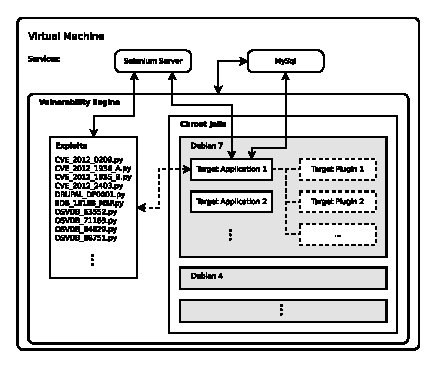
\includegraphics[scale=1.17]{system_diagram.eps}
\end{center}
\caption{System Diagram}
\end{figure}


\subsection{Engine}
It is the job of the {\bf Engine} to match exploits with target modules and actually perform setup, configuration, and teardown work. The Engine will prepare a \texttt{chroot} environment by mounting target operating system and web application folders under the environment, load a stored MySQL database, install the appropriate XDebug PHP debugger configuration file, start the web server, and eventually perform cleanup operations associated with these steps. 

To illustrate the role of the engine, the following lines in the first use case are relevant:
\begin{description}
  \item[Line 5] {\tt \footnotesize    engine = Engine(Exploit(), config)} \\ A new engine instance is constructed with an exploit instance and system configuration as arguments.
  \item[Line 6] {\tt \footnotesize     engine.startup()} \\The engine creates a {\tt chroot} environment on the host system to which the target application is copied. The choice of application is determined by the 'Target' attribute in the exploit instance. 
  \item[Lines 7 \& 9] {\tt \footnotesize engine.xdebug\_autotrace\_on()\\ engine.xdebug\_autotrace\_on()}\\The engine can modify the state of the trace collection in X\_Debug to ensure that only the trace pertinent to the exploitation is collected.
  \item[Line 10] {\tt \footnotesize engine.shutdown()}\\This cleanup code unmounts the {\tt chroot} environment and returns the corpus environment back to an un-altered state.
\end{description}



%\begin{figure}[!tp]
%\begin{center}
%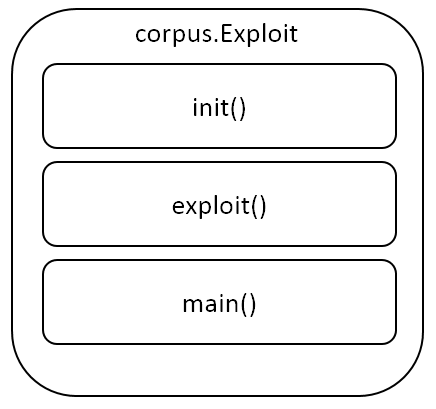
\includegraphics[scale=.5]{Corpus_Exploit.PNG}
%\end{center}
%\caption{Exploit Structure}
%\end{figure}


\subsection{Target module}
The {\bf Target} module contains logic relevant to deploying the application target that the exploit may be applied to.  More specifically, an application target is a specific version of a PHP web application such as WordPress. A copy of the target application with a typical configuration is always loaded before any exploit script is run.  For each application, an initialization script is written to provide the {\bf Engine} with the proper details for the installation; for example:

\begin{minipage}{\textwidth}
{\tt \footnotesize
%\begin{verbatim}
\begin{lstlisting}
name = "Wordpress 3.3.1"
application_dir_mapping = ...
    [get_path("application"), ...
     "/var/www"]
database_filename = ...
    get_path("database.sql")
database_name = "wordpress_3_3_1_A"
chroot_environment = "Debian7"
\end{lstlisting}
%\end{verbatim}
} 
\end{minipage}


Some large web applications, such as WordPress, have many plugins that have vulnerabilities themselves. Therefore, {\bf Target} modules also allow for the inclusion of plugins in the exploit framework. Both targets and target plugins are resolved against the exploit attributes by the Engine during the setup process. 


\subsection{Exploit class}
The {\bf Exploit} class is the superclass for each exploit in the corpus, defining interfaces and attributes that the engine uses to manage the environment and exploitation. The Exploit class is structured such that exploits can be written with concise code functions. Each exploit is simply a subclass of Exploit residing in its own Python file. This class ensures that the Selenium driver is properly initialized and bound to each exploit, and that each exploit script can define actions to take upon installation.

The separation between targets and exploits allows for those unfamiliar with the framework to develop exploits without being concerned with the application or environment setup process, allowing BugBox to be extended without having to learn the intricacies of the entire framework.\par
 
Metadata for the exploit module is provided by its attribute dictionary. In it, we declare the name, description, references, target, type, and wiki page for the exploit .  The name is the identifier specified in one of the online databases of vulnerabilities mentioned earlier in this paper.  The description is a brief statement of what the exploit is supposed to do, because the name is typically does not describe what type of exploit is being applied.  The Target is the web application module which is being used for the exploit. The type is the type of exploit being conducted (such as XSS). The wiki page directs a user to a page where auxiliary information about the exploit or script is recorded. The Query module, also part of BugBox, allows for this metadata queried across all exploits (as described in the use cases).

Here is an example body of an exploit procedure used for a simple XSS attack. Scripting the exploit only requires instantiating the Selenium driver and submitting a request on the WordPress site with the payload: 

\begin{minipage}{\textwidth}
{\tt \footnotesize
%\begin{verbatim}
\begin{lstlisting}
payload = "<a href=\"#\" title=\"XSS	\
          http:" //example.com/				\
          onmouseover=eval(" 					\
          "unescape(/%61%6c%65%"			\
          "72%74%28%31%29%3b%61"			\
          "%6c%65%72%74%28%32"				\
          "%29%3b%61%6c%65%72"				\
          "%74%28%33%29%3b/." 				\
          "source))//\">XSS</a>"

driver = self.create_selenium_driver()

driver.get(...
     "http://localhost/wordpress/?p=1")
get = driver.find_element_by_id
get("author").send_keys(...
     "selenium script")
get("email").send_keys(...
    "selenium@python.org")
get("url").send_keys("www.python.org")
get("comment").send_keys(payload)
get("submit").click()
\end{lstlisting}
%\end{verbatim}
}
\end{minipage}


\subsection {Cleanup and maintenance}


Functionality that performs cleanup and maintenance are included in BugBox to ensure that results based on the framework are reproducible. There are many changes that occur in the system over the course of the exploit cycle that will potentially need to be eliminated. Even changes that would normally seem innocuous, like recording events to a log file, have the potential to at some point change program behaviour.  

Since the {\tt chroot} environments on the host machine are represented as directories in the host filesystem, simple scripts are used to maintain them.  Scripts using {\tt rsync} are employed to periodically overwrite the {\tt chroot} jails with fresh copies to maintain the integrity of their operating systems. Exploit scripts are also responsible for removing their own side-effects from the target application. For instance, many exploits upload an arbitrary file to be executed by the webserver. The exploit classes can implement a cleanup method which has direct access to the target filesystem, allowing for the environment to be restored to its pre-exploitation state. 

\section {Lessons learned}

In developing BugBox, we learned four key lessons, involving: the need for multiple versions of environments, the utility of visual aids to speed up exploit script development, the importance of representative sampling, and the benefits of building a modular system.\par

Being able to install web applications onto multiple operating system environments is a critical factor in corpus development.  When creating a corpus, a wide variety of examples is required, including web application versions that are outdated.  Some of these outdated applications have dependencies on older software versions, which are only included with obsolete Linux distributions. For this reason, we ensured that BugBox supported the use of multiple environments with different Linux distributions.\par

Exploit script development is a repetitive and necessary process. We found that the instant feedback provided by the Selenium visual framework allowed us to more rapidly create exploit scripts.  Being able to visually monitor the execution of the scripts allows developers to efficiently pinpoint errors, streamlining script generation.  \par

Originally, when collecting samples for our corpus, we failed to focus on collecting a representative sample across independent variables such as vulnerability type and age. Having a proper sample is important when evaluating exploit prevention techniques~\cite{testbedpaper} or analyzing source code metrics, to ensure that the result is fair and representative. We will remediate this by collecting new vulnerabilities and stratifying the sample across these variables, and we recommend that future teams collecting vulnerability data apply proper sampling procedures as early in the process as possible.\par

In our original implementation of this framework, each vulnerability was permanently installed on a separate virtual machine image. We found that introducing new processes which affected the entire corpus (such as beginning to collect execution traces) required large amounts of labor, repeating the process for each VM. The BugBox framework automatically installs vulnerable applications onto a test environment which can be customized at any time, speeding up these tasks. Repetitive research tasks are further facilitated by the use of Python as a layer of abstraction above the target environment, target application, and exploits.

\subsection {Ethical Considerations}
BugBox is a powerful tool for researchers which could potentially provide a foundation for a fully automated attack platform for malicious attackers.  With this in mind, we implemented measures to decrease the potential for malicious use of our system through two rules:

First, no zero-day exploits will be added or accepted to the main distribution of BugBox. Because BugBox is used for research and education, it is sufficient to limit the scope of BugBox to historical vulnerabilities which are already cataloged in any well-known vulnerability or exploit database.
Next, all new exploits created or accepted for the framework will only include functionality necessary to test the vulnerability in the BugBox environment and will not contain code that is tailored toward a general-purpose attack.  This provides more overhead for an attacker considering this tool for malicious use, thus impeding a ``script kiddie'' from using the tool maliciously.  Significant modification would be required for an exploit script to carry an actual malicious payload or target vulnerable applications in an unpredictable, real-life environment.
Although it is beyond anyone's reach to prevent a user from maliciously using any vulnerability or exploit repository, including our own, by implementing these measures, we seek to limit the audience of malicious users.

\section{Future work}
We plan to implement additional features for controlling trace collection through cookie manipulation via XDebug. This will reduce the collection of insignificant interactions (such as pre-exploit setup requests) and provide a more refined break-down of the exploitation process, as traces would be grouped by HTTP request.

The exploits in the corpus have no standard method for selecting the payload which will used in the attack. Since studies on intrusion detection or prevention systems may be sensitive to the payload type and encoding, researchers may desire finer-grained control over this property. The Metasploit Framework has a robust system for managing exploits along with their payloads and encodings, serving as a model for implementing this if needed.

More information on obtaining BugBox for research use is available from our website: \url{http://seam.cs.umd.edu/Projects/BugBox/}. BugBox is designed to work on the Debian GNU/Linux and compatible distributions. The framework can be obtained in the form of a package which can be installed on an existing system. The system must have sufficient storage (roughly 4 GB per OS environment, and up to 2 GB for the application, engine, and exploit sources) with access rights to use run Linux {\tt chroot} jails.  Dependencies for the BugBox host system include MySQL, Selenium Server, and \texttt{debootstrap}. Community contributions will be key to building a corpus of sufficient size, therefore, community members may contribute BugBox exploit and target modules as described on the website. The framework is distributed under an open-source license. Because the corpus is composed entirely of open-source applications, target modules will be distributed under the application's respective license.

\section*{Acknowledgments}

The authors thank the United States Office of Naval Research for its support for this research under contract N000141210147.

{\footnotesize \bibliographystyle{acm}
\bibliography{ref}}

\end{document}
